\documentclass{article}

\usepackage{graphicx}
\usepackage{tikz}
\usepackage{tikzsymbols}
\usetikzlibrary{calc,patterns,shapes.geometric}
\pagestyle{empty}
\usepackage[margin=0pt]{geometry}
\geometry{papersize={14in,12in}}

\def\centerarc[#1](#2)(#3:#4:#5){\draw[#1] ($(#2)+({#5*cos(#3)},{#5*sin(#3)})$) arc (#3:#4:#5);}

\begin{document}
	\begin{figure}
		\centering
		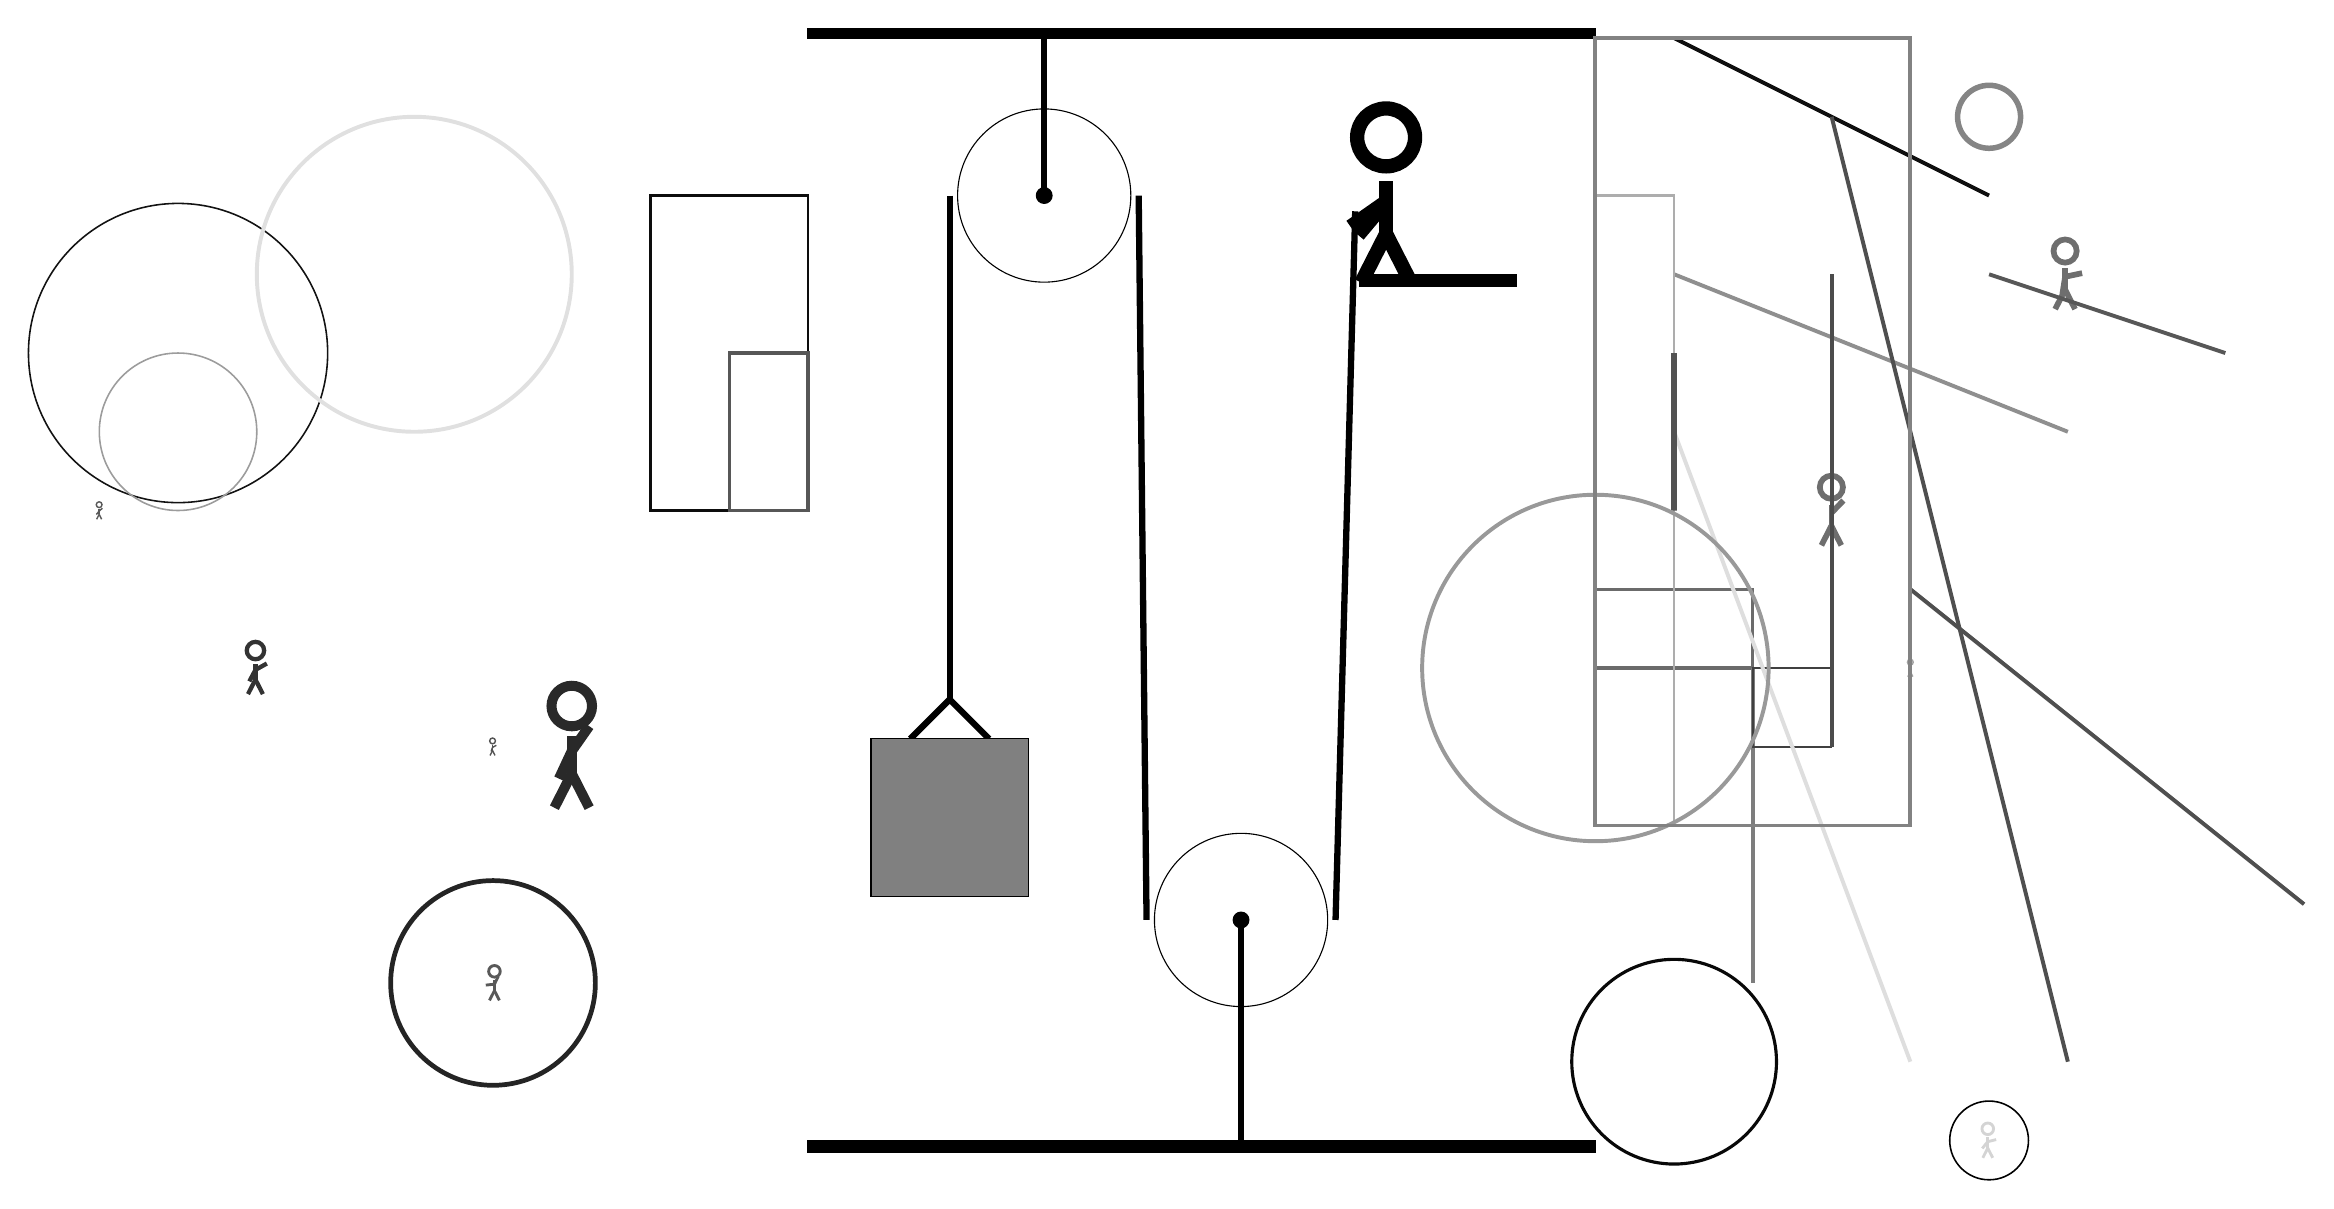
\begin{tikzpicture}
			%%%%% START %%%%%
			
			\draw[fill=black] (-2, 14) rectangle (8, 14.125);
			
			\draw (3.5, 2.8) circle (1.1);
			\draw[fill=black] (3.5, 2.8) circle (0.1);
			\draw[line width=0.8mm] (3.5, 2.8) -- (3.5, 0);
			
			\draw[line width=0.5mm, color=black!44](9, 11) -- (14, 9);
			
			\draw[line width=0.4mm, color=black!58] (8, 6) rectangle (10, 7);
			\node[line width=0.3mm, color=black!37] at (12, 6) {\Strichmaxerl[1][80][87]};
			\draw[line width=0.5mm, color=black!94](9, 14) -- (13, 12);
			\node[line width=0.7mm, color=black!57] at (11, 8) {\Strichmaxerl[4][90][46]};
			\draw [line width=0.2mm, color=black!93](-10, 10) circle (1.9);
			
			\node[line width=0.3mm, color=black!67] at (-6, 5) {\Strichmaxerl[1][71][28]};
			
			\draw [line width=0.2mm, color=black!100](13, 0) circle (0.5);
			\node[line width=0.2mm, color=black!57] at (14, 11) {\Strichmaxerl[4][81][12]};
			
			\node[line width=0.7mm, color=black!17] at (13, 0) {\Strichmaxerl[2][51][14]};
			
			\draw[line width=0.5mm, color=black!51](10, 2) -- (10, 6);
			\draw [line width=0.2mm, color=black!39](-10, 9) circle (1.0);
			\draw[line width=0.2mm, color=black!75] (10, 6) rectangle (11, 5);
			\draw [line width=0.6mm, color=black!86](-6, 2) circle (1.3);
			\draw[line width=0.5mm, color=black!13](9, 9) -- (12, 1);
			\node[line width=0.4mm, color=black!80] at (-9, 6) {\Strichmaxerl[3][62][29]};
			
			\draw[line width=0.5mm, color=black!70](11, 5) -- (11, 11);
			\draw[line width=0.3mm, color=black!32] (9, 12) rectangle (8, 4);
			\draw[line width=0.5mm, color=black!69](12, 7) -- (17, 3);
			\node[line width=0.7mm, color=black!84] at (-5, 5) {\Strichmaxerl[7][65][55]};
			\node[line width=0.2mm, color=black!65] at (-6, 2) {\Strichmaxerl[2][6][64]};
			
			\draw[line width=0.5mm, color=black!69](11, 13) -- (14, 1);
			
			\draw [line width=0.4mm, color=black!97](9, 1) circle (1.3);
			\draw[line width=0.7mm, color=black!68] (9, 8) rectangle (9, 10);
			\draw[line width=0.3mm, color=black!95] (-2, 12) rectangle (-4, 8);
			
			\draw [line width=0.5mm, color=black!40](8, 6) circle (2.2);
			
			\draw [line width=0.7mm, color=black!48](13, 13) circle (0.4);
			\draw[line width=0.5mm, color=black!66](13, 11) -- (16, 10);
			
			\draw [line width=0.5mm, color=black!12](-7, 11) circle (2.0);
			\node[line width=0.7mm, color=black!65] at (-11, 8) {\Strichmaxerl[1][50][42]};
			\draw[line width=0.5mm, color=black!49] (8, 4) rectangle (12, 14);
			
			\draw[line width=0.4mm, color=black!66] (-3, 10) rectangle (-2, 8);
			
			\draw (1, 12) circle (1.1);
			\draw[fill=black] (1, 12) circle (0.1);
			\draw[line width=0.8mm] (1, 14) -- (1, 12);
			
			\draw[line width=0.8mm](-0.7, 5.1) --  (-0.2, 5.6) -- (0.3, 5.1);
			\draw[fill=black!50] (-1.2, 5.1) rectangle (0.8, 3.1);
			
			\draw[line width=0.8mm](-0.2, 12) -- (-0.2, 5.6);
			\centerarc[line width=0.8mm](1, 12)(180:0:1.2000000000000002)
			\draw[line width=0.8mm](2.2, 12) -- (2.3, 2.8);
			\centerarc[line width=0.8mm](3.5, 2.8)(180:360:1.2000000000000002)
			\draw[line width=0.8mm](4.7, 2.8) -- (4.95, 11.8);
			
			\node at (5.3, 12) {\Strichmaxerl[10][35][-130]};
			\draw[fill=black] (5, 11) rectangle (7, 10.85);
			
			\draw[fill=black] (-2, 0) rectangle (8, -0.15);
			
			%%%%% END %%%%%
		\end{tikzpicture}
	\end{figure}	
\end{document}